%%%%%%%%%%%%%%%%%%%%%%%%%%%%%%%%%%%%%%%%%
% Beamer Presentation
% LaTeX Template
% Version 1.0 (10/11/12)
%
% This template has been downloaded from:
% http://www.LaTeXTemplates.com
%
% License:
% CC BY-NC-SA 3.0 (http://creativecommons.org/licenses/by-nc-sa/3.0/)
%
%%%%%%%%%%%%%%%%%%%%%%%%%%%%%%%%%%%%%%%%%

%----------------------------------------------------------------------------------------
%   PACKAGES AND THEMES
%----------------------------------------------------------------------------------------

\documentclass{beamer}

\mode<presentation> {

  % The Beamer class comes with a number of default slide themes
  % which change the colors and layouts of slides. Below this is a list
  % of all the themes, uncomment each in turn to see what they look like.

  %\usetheme{default}
  %\usetheme{AnnArbor}
  %\usetheme{Antibes}
  %\usetheme{Bergen}
  %\usetheme{Berkeley}
  %\usetheme{Berlin}
  %\usetheme{Boadilla}
  \usetheme{CambridgeUS}
  %\usetheme{Copenhagen}
  %\usetheme{Darmstadt}
  %\usetheme{Dresden}
  %\usetheme{Frankfurt}
  %\usetheme{Goettingen}
  %\usetheme{Hannover}
  %\usetheme{Ilmenau}
  %\usetheme{JuanLesPins}
  %\usetheme{Luebeck}
  %\usetheme{Madrid}
  %\usetheme{Malmoe}
  %\usetheme{Marburg}
  %\usetheme{Montpellier}
  %\usetheme{PaloAlto}
  %\usetheme{Pittsburgh}
  %\usetheme{Rochester}
  %\usetheme{Singapore}
  %\usetheme{Szeged}
  %\usetheme{Warsaw}

  % As well as themes, the Beamer class has a number of color themes
  % for any slide theme. Uncomment each of these in turn to see how it
  % changes the colors of your current slide theme.

  %\usecolortheme{albatross}
  %\usecolortheme{beaver}
  %\usecolortheme{beetle}
  %\usecolortheme{crane}
  %\usecolortheme{dolphin}
  \usecolortheme{dove}
  %\usecolortheme{fly}
  %\usecolortheme{lily}
  %\usecolortheme{orchid}
  %\usecolortheme{rose}
  %\usecolortheme{seagull}
  %\usecolortheme{seahorse}
  %\usecolortheme{whale}
  %\usecolortheme{wolverine}

  %\setbeamertemplate{footline} % To remove the footer line in all slides uncomment this line
  %\setbeamertemplate{footline}[page number] % To replace the footer line in all slides with a simple slide count uncomment this line

  %\setbeamertemplate{navigation symbols}{} % To remove the navigation symbols from the bottom of all slides uncomment this line
}

\usepackage{graphicx} % Allows including images
\usepackage{booktabs} % Allows the use of \toprule, \midrule and \bottomrule in tables
\usepackage{listings}
\usepackage{tikz}
\usepackage{subcaption}
\usepackage[scientific-notation=true]{siunitx}

%----------------------------------------------------------------------------------------
%   TITLE PAGE
%----------------------------------------------------------------------------------------

\title[Learning Job Run-Times in HPC Systems]{Learning Job Run-Times in HPC Systems} % The short title appears at the bottom of every slide, the full title is only on the title page

\author{Valentin Reis} % Your name
\institute[LIG AMA] % Your institution as it will appear on the bottom of every slide, may be shorthand to save space
{
  %MoSIG M1 at Joseph Fourier University\\ % Your institution for the ttle page
  LIG, AMA Team.\\ % Your institution for the title page
  Under supervision of: Eric Gaussier and Denis Trystram. \\
  \medskip
  %\textit\t{valentin.reis@gmail.com} % Your email address
}
\date{\today} % Date, can be changed to a custom date

\begin{document}
\begin{frame}
  \titlepage % Print the title page as the first slide
\end{frame}

%\begin{frame}
  %\frametitle{Overview} % Table of contents slide, comment this block out to remove it
  %\tableofcontents % Throughout your presentation, if you choose to use \section{} and \subsection{} commands, these will automatically be printed on this slide as an overview of your presentation
%\end{frame}


\section{Introduction}
\label{sec:introduction}

\label{sub:scheduling_in_hpc_systems}

\begin{frame}
  \frametitle{Resource Management in HPC Systems}

  High Performance Computing is:
  \centering

    \hfill
    \parbox{.70\textwidth}{
      \begin{itemize}
    \item Complex architectures.
    \item Uncertain data.
      \end{itemize}}

\end{frame}


\begin{frame}
  \frametitle{Jobs}

  This is a job:
  \begin{figure}[H]
          \centerin
          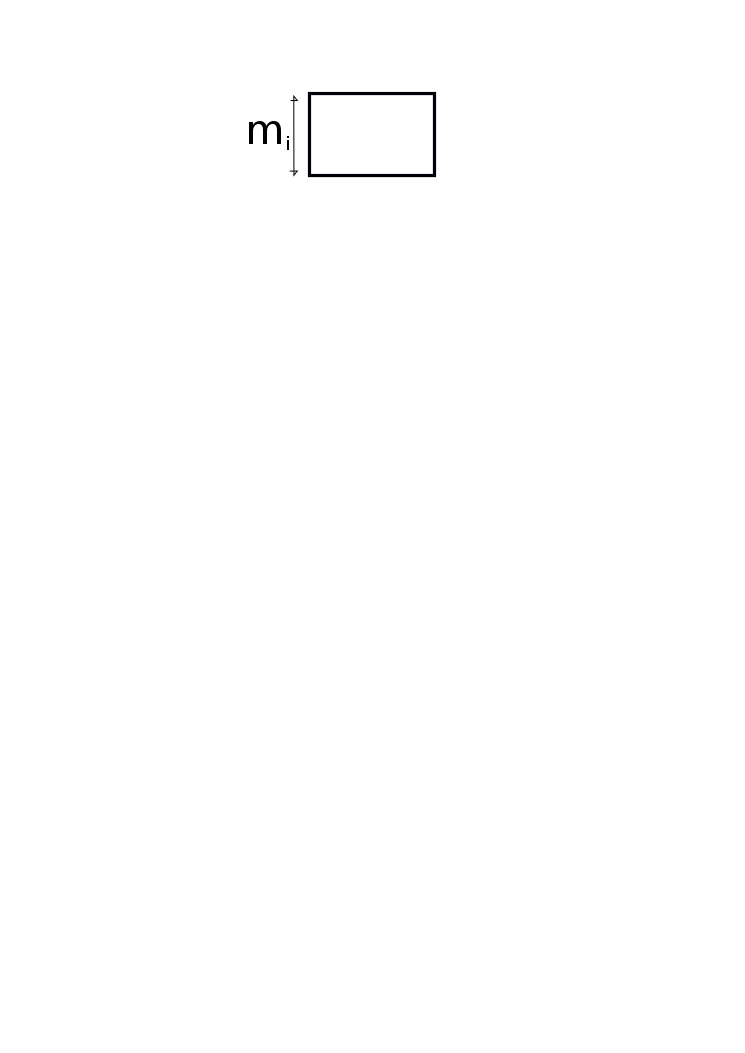
\includegraphics[width=\textwidth]{job.png}
          \caption{Caption}
          \label{fig:job_jpg}
  \end{figure}

\end{frame}
\label{sub:jobs}


\begin{frame}
  \frametitle{Jobs}

  This is a job on a system:
  \begin{figure}[H]
          \centerin
          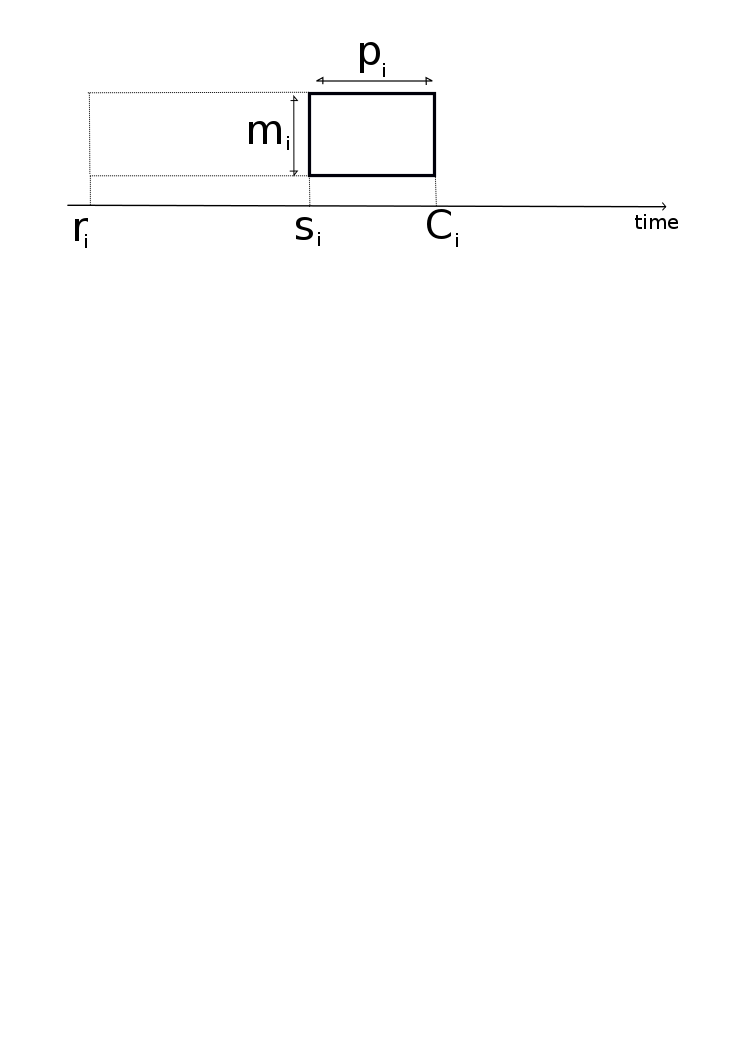
\includegraphics[width=\textwidth]{job_system.png}
          \caption{Caption}
          \label{fig:job_jpg}
  \end{figure}

\end{frame}
\label{sub:jobs}


% subsection jobs (end)

\label{sub:objectives}
\begin{frame}
  \frametitle{Objectives}
  \centering
  \begin{figure}
  \begin{itemize}
    \item $\sum_{i=0}^{i=n} C_i$ (Minsum)
    \item $\max_{i=0}^{i=n} C_i$ (Makespan)
    \item $\sum_{i=0}^{i=n} C_i-r_i$ (Flow Time)
    \item $\sum_{i=0}^{i=n} \frac{C_i-r_i}{C_i-\sigma(i)}$ (Sum Stretch)
    \item $\max_{i=0}^{i=n} \frac{C_i-r_i}{C_i-\sigma(i)}$ (Max Stretch)
    \item Many others
    \item And their combinations!
  \end{itemize}
  \end{figure}
  \pause
  And: functional constraints. \textbf{no starvation}, please!
\end{frame}


\begin{frame}<1>[label=frame1]
  \frametitle{What problem is it?}
  \begin{itemize}
    \item<1-> Offline Scheduling, a.k.a.\ strip packing? \onslide<2->{-- no}
    \item<3-> Online Scheduling? \onslide<4->{-- no}
    \item<5-> Online Scheduling under Uncertainty \onslide<6->{-- yes!}
  \end{itemize}
\end{frame}

\begin{frame}
  \frametitle{Offline Scheduling}
  \begin{figure}[H]
          \centering
          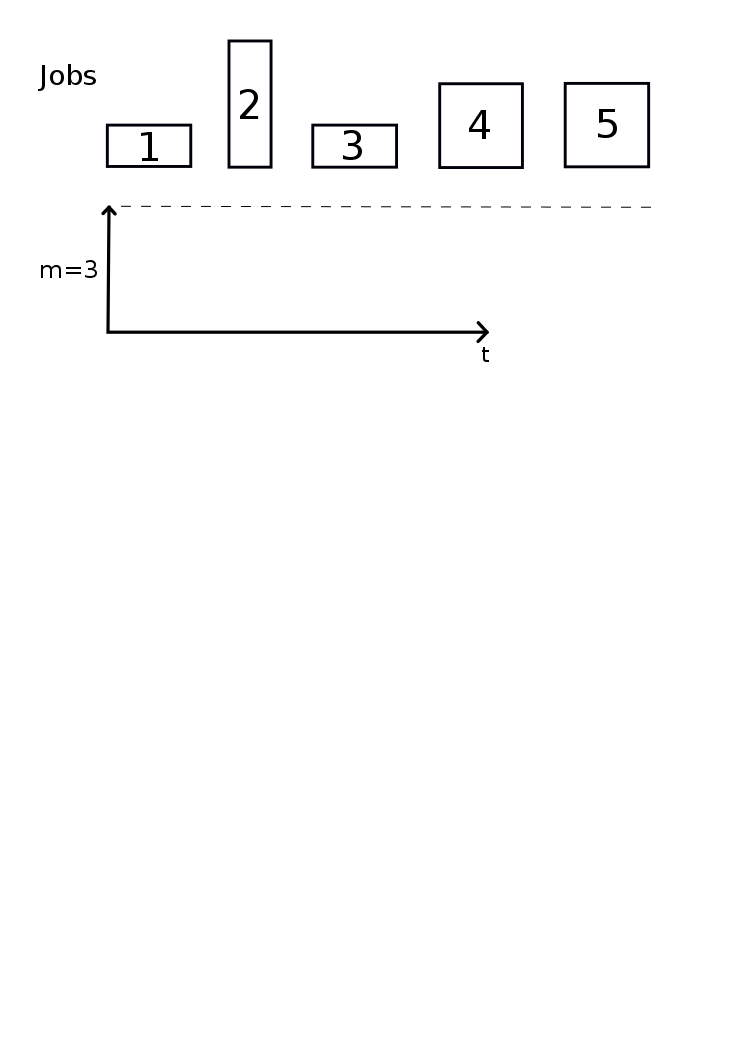
\includegraphics[width=\textwidth]{offline.png}
          \caption{Caption}
          \label{fig:offline_png}
  \end{figure}

\end{frame}
\begin{frame}
  \frametitle{Offline Scheduling}
  \begin{figure}[H]
          \centering
          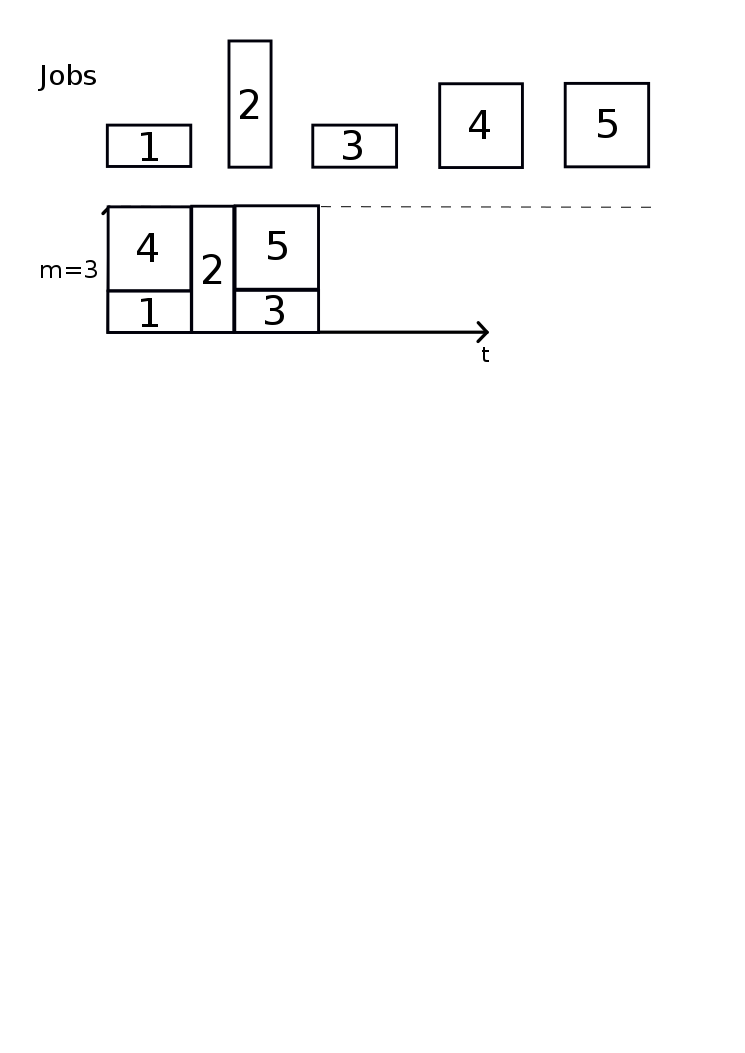
\includegraphics[width=\textwidth]{offline2.png}
          \caption{Caption}
          \label{fig:offline2_png}
  \end{figure}

\end{frame}

\againframe<1-3>{frame1}

\begin{frame}
  \frametitle{Online Scheduling}
  \begin{figure}[H]
          \centering
          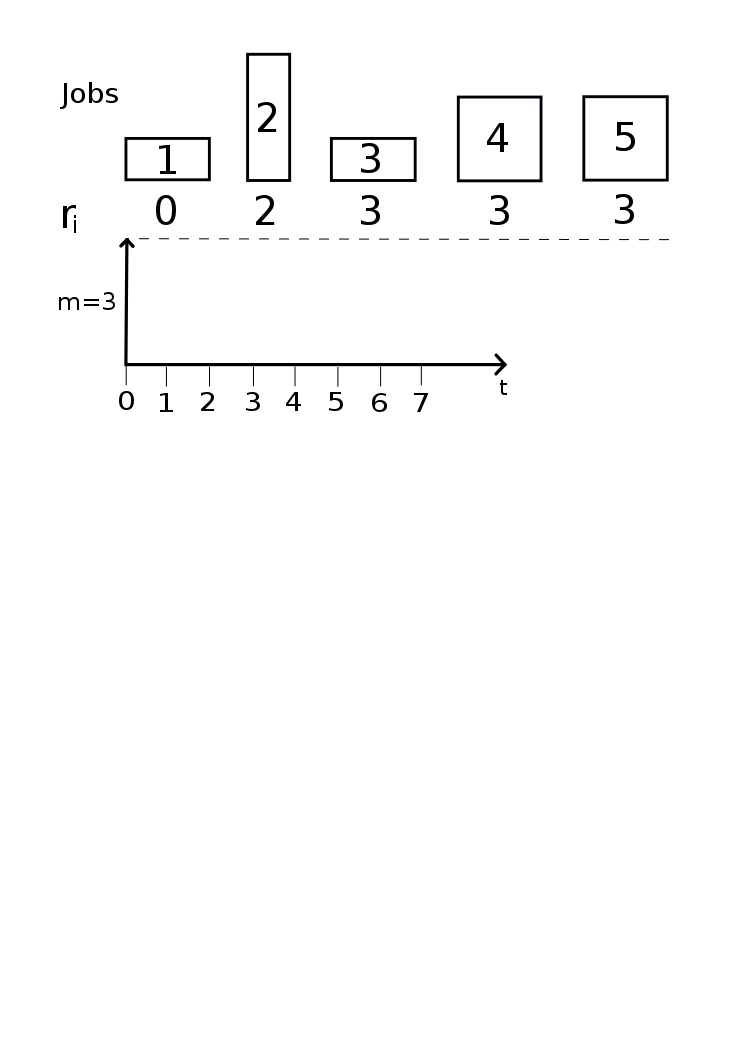
\includegraphics[width=\textwidth]{online.png}
          \caption{Caption}
          \label{fig:online_png}
  \end{figure}

\end{frame}


\begin{frame}
  \frametitle{Online Scheduling}
  \begin{figure}[H]
          \centering
          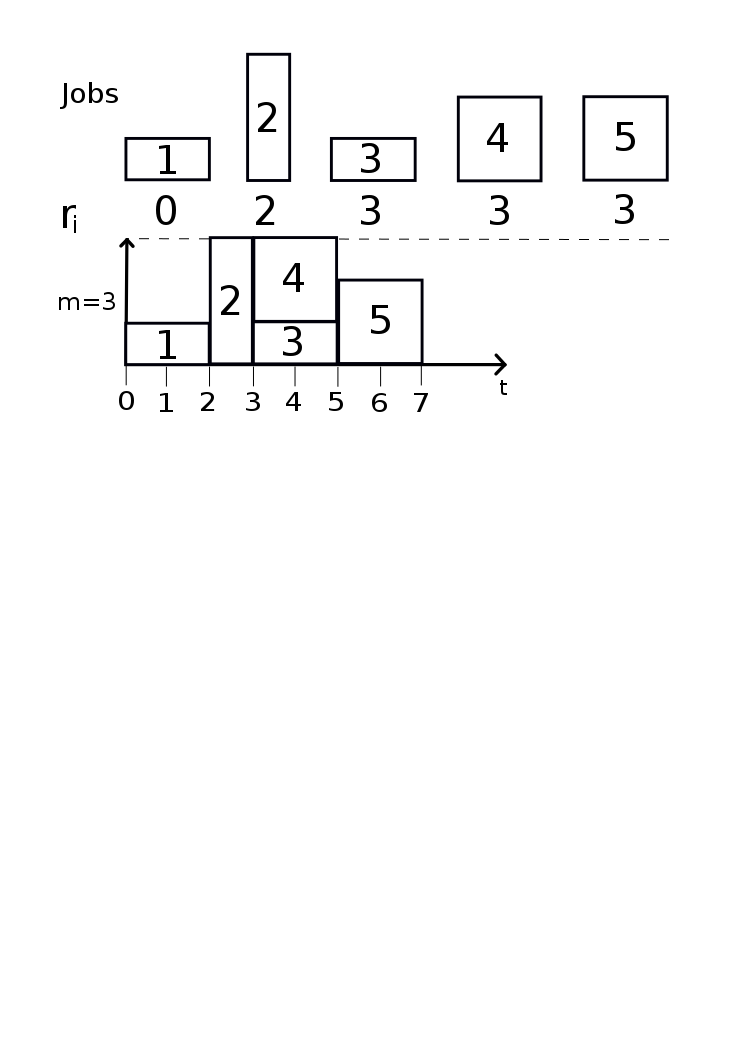
\includegraphics[width=\textwidth]{online2.png}
          \caption{Caption}
          \label{fig:online2_png}
  \end{figure}

\end{frame}


\begin{frame}
  \frametitle{Uncertainty in Run-times}

\begin{figure}[]
    \centering
    \begin{subfigure}{0.4\textwidth}
        \centering
        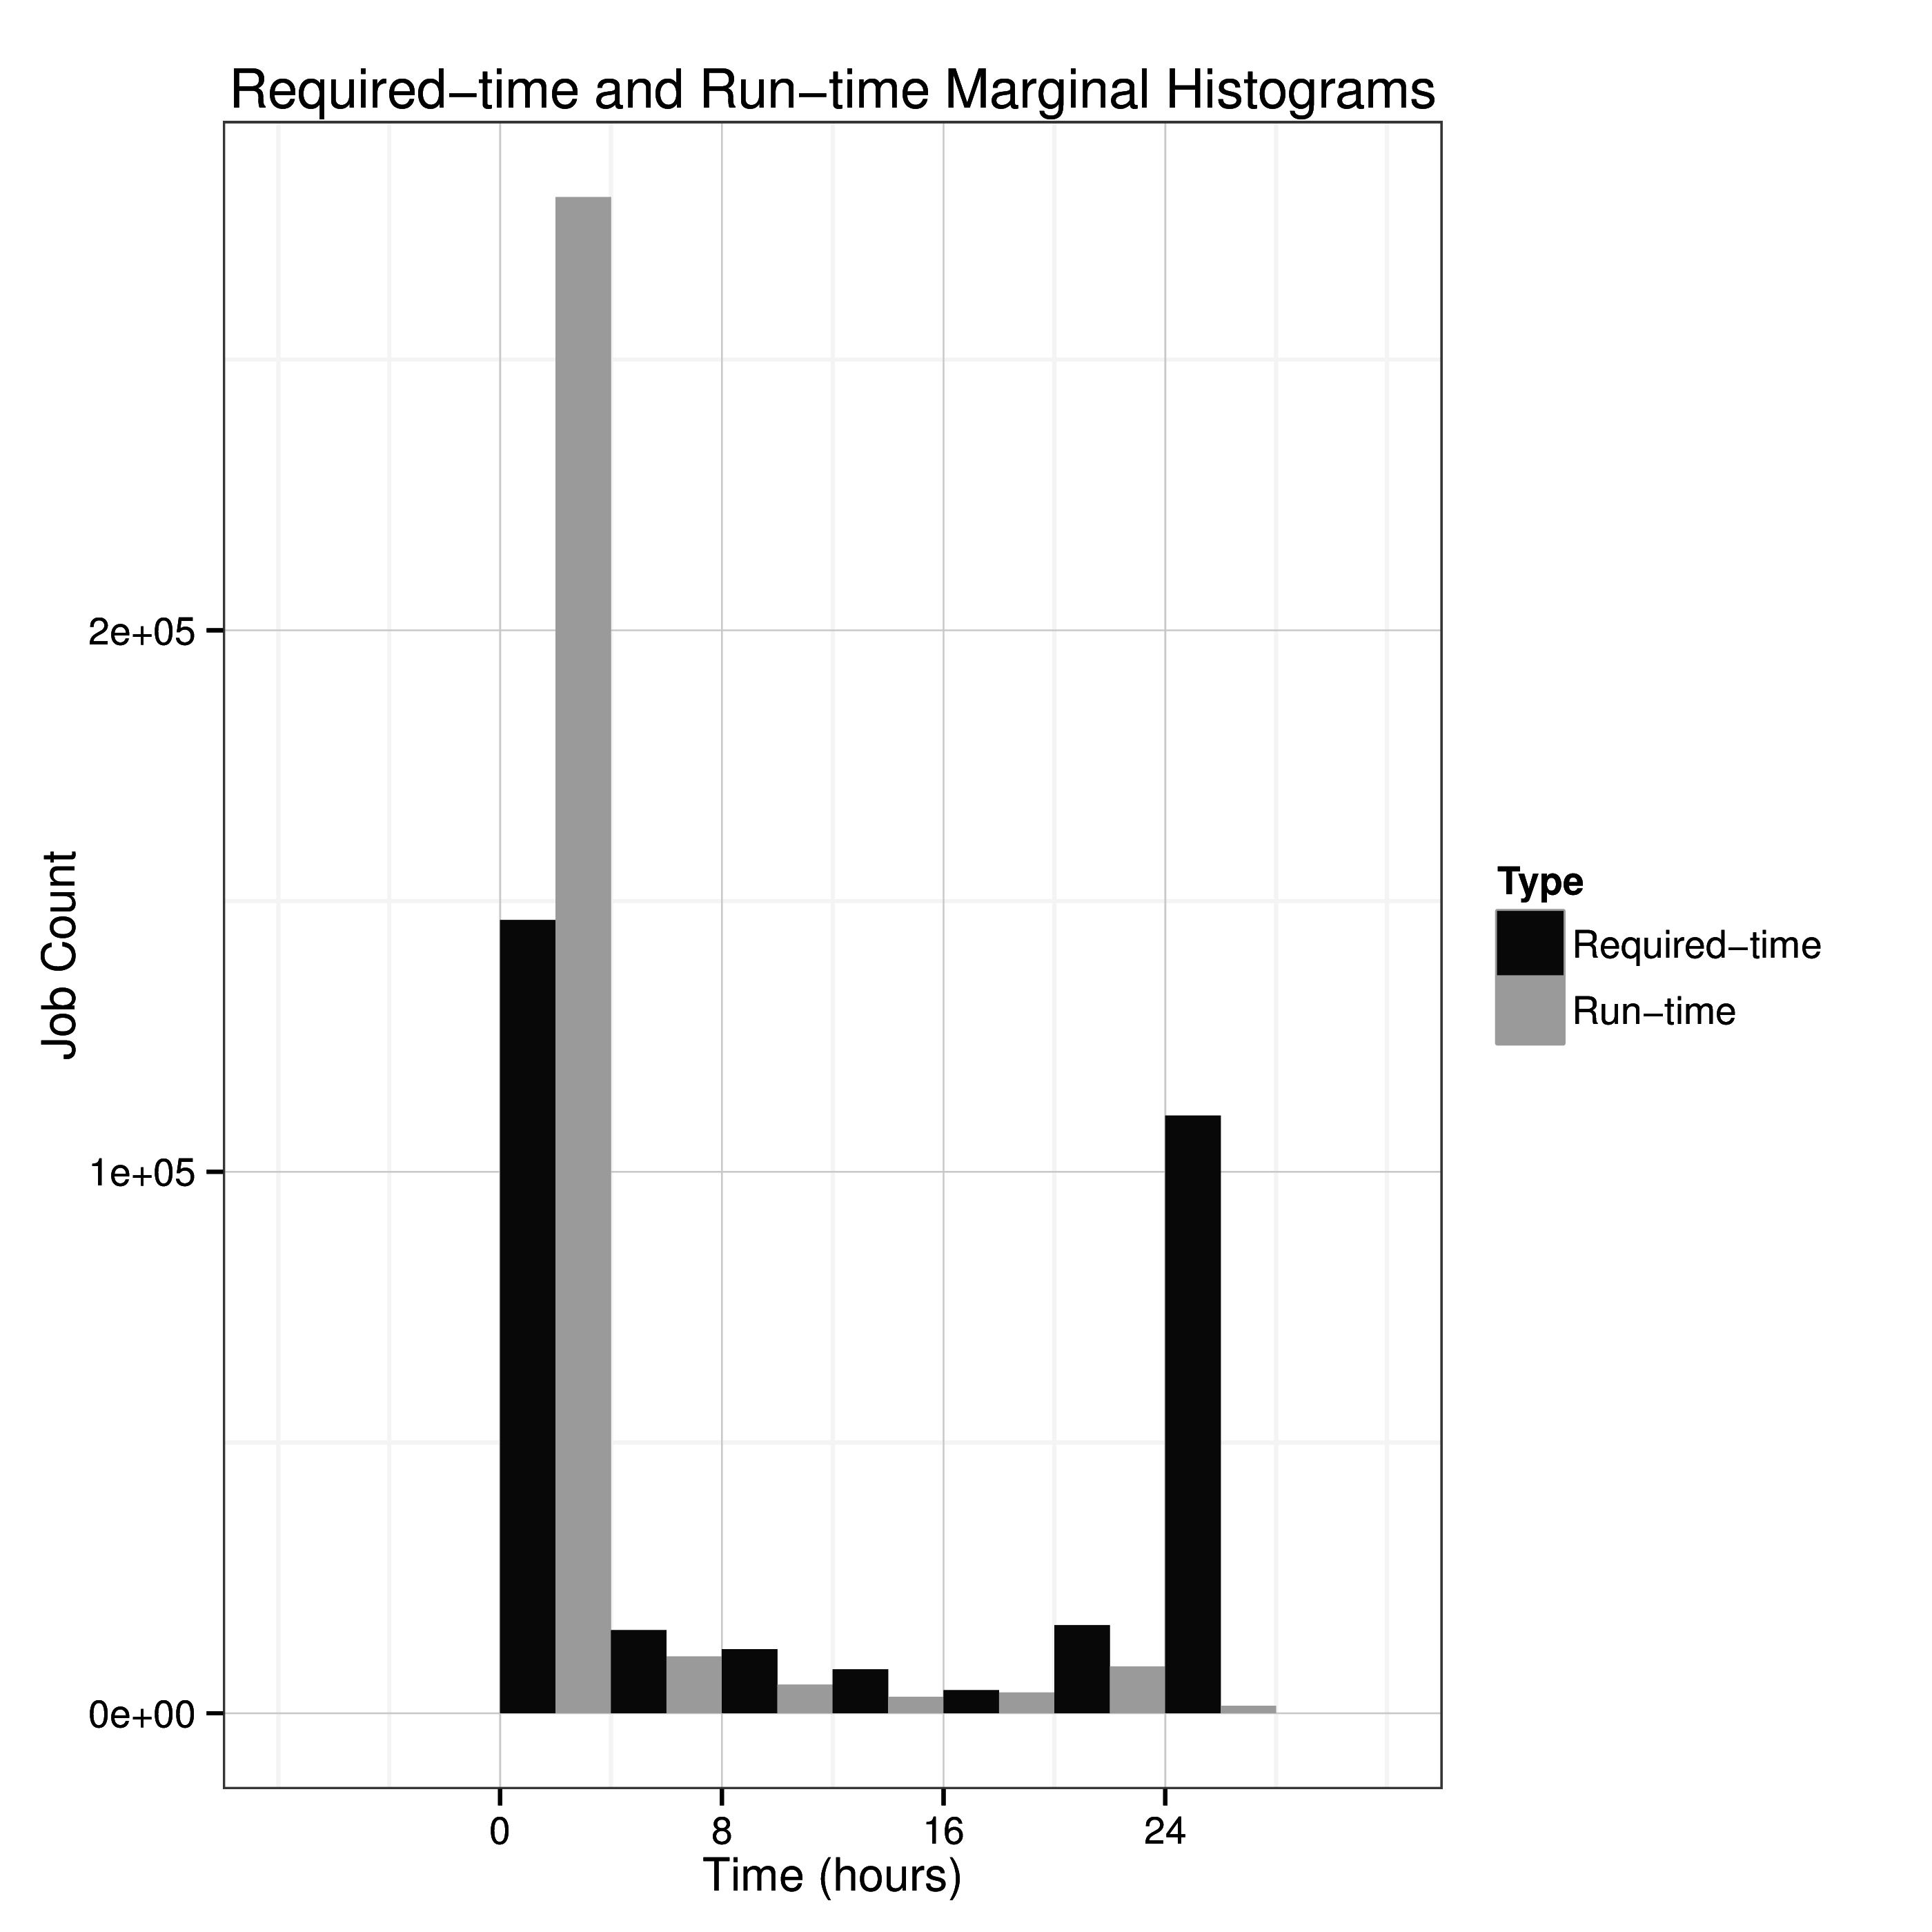
\includegraphics[width=0.9\textwidth]{../report/reqrun-0.png}
        \caption{Marginal}
        \label{fig:_report_reqrun_0_png}
    \end{subfigure}
    \begin{subfigure}{0.4\textwidth}
        \centering
        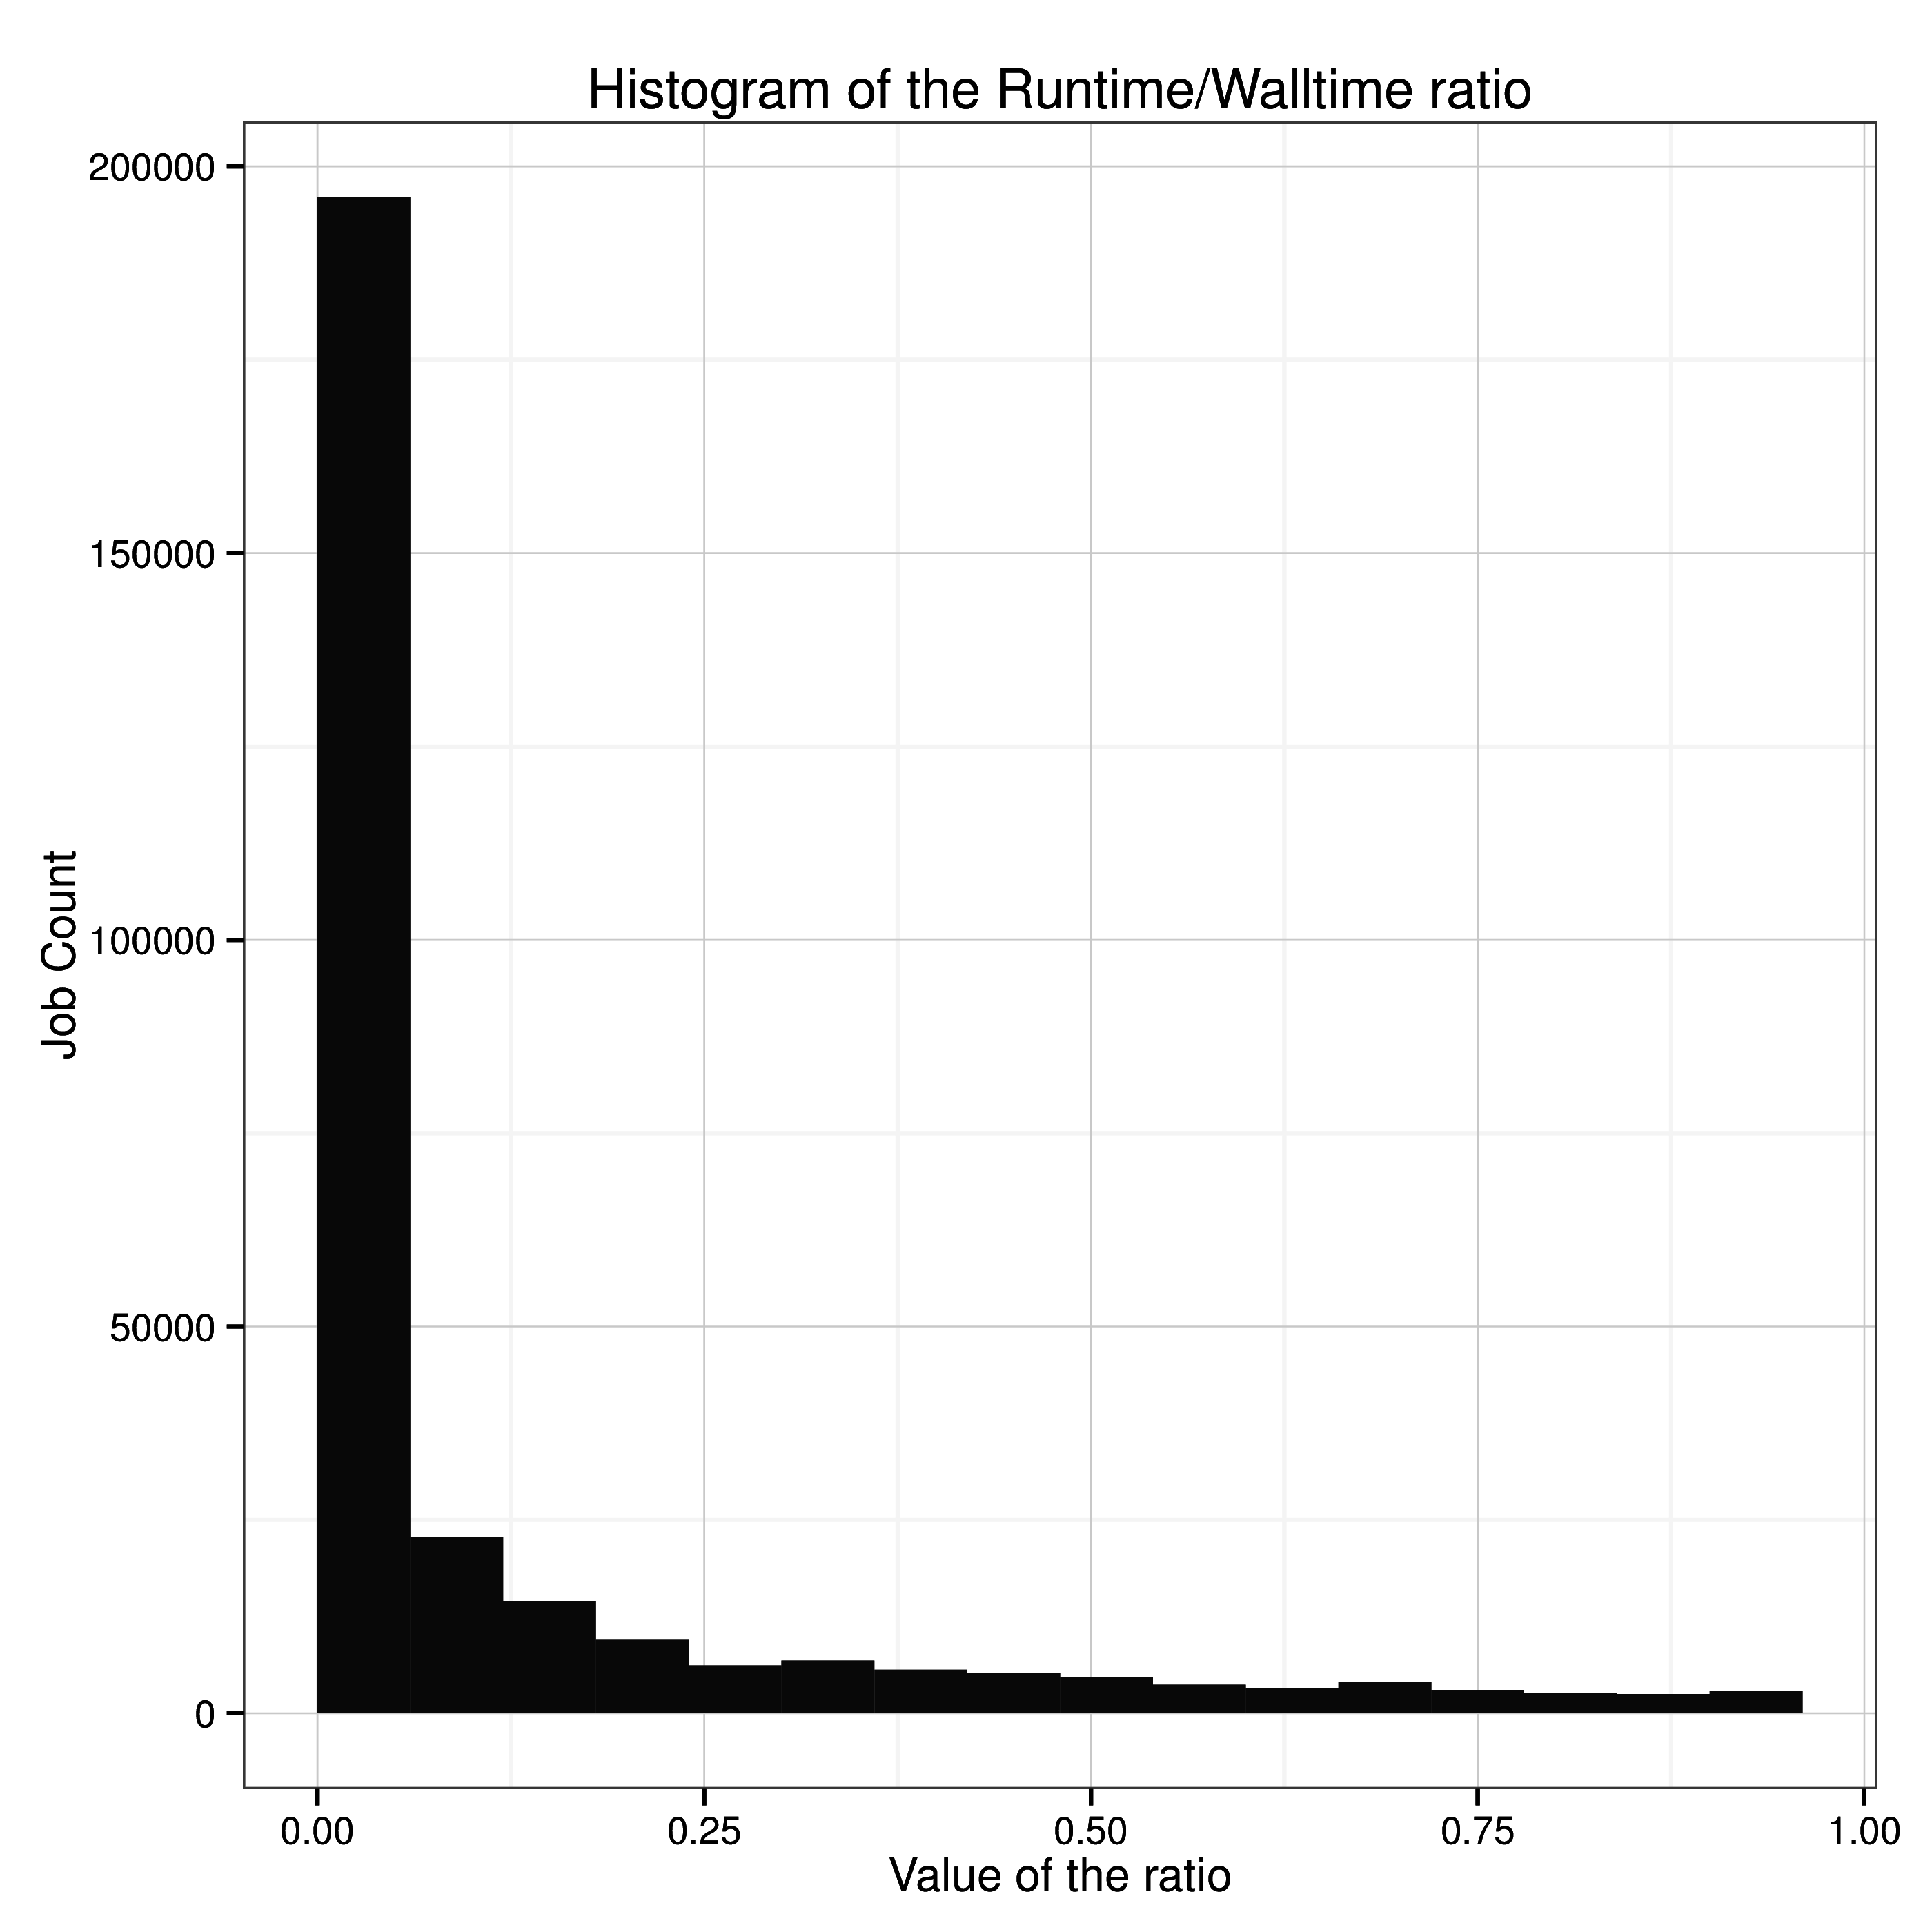
\includegraphics[width=0.9\textwidth]{../report/reqrun-1.png}
        \caption{Ratio}
        \label{fig:_report_reqrun_1_png}
    \end{subfigure}
    \label{fig:global_label}
\end{figure}


\end{frame}

\againframe<3-6>{frame1}

\begin{frame}
  \frametitle{Online Scheduling under Uncertainty}
  \begin{figure}[H]
          \centering
          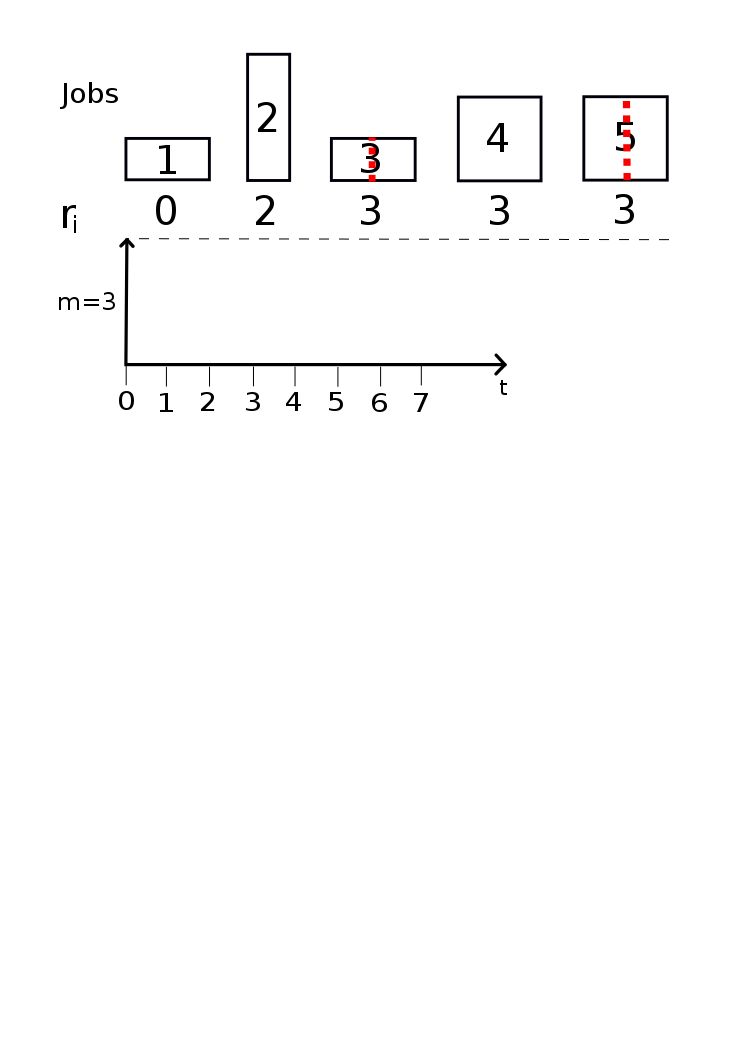
\includegraphics[width=\textwidth]{uncertain.png}
          \caption{Caption}
          \label{fig:online_png}
  \end{figure}

\end{frame}


\begin{frame}
  \frametitle{Online Scheduling under Uncertainty}
  \begin{figure}[H]
          \centering
          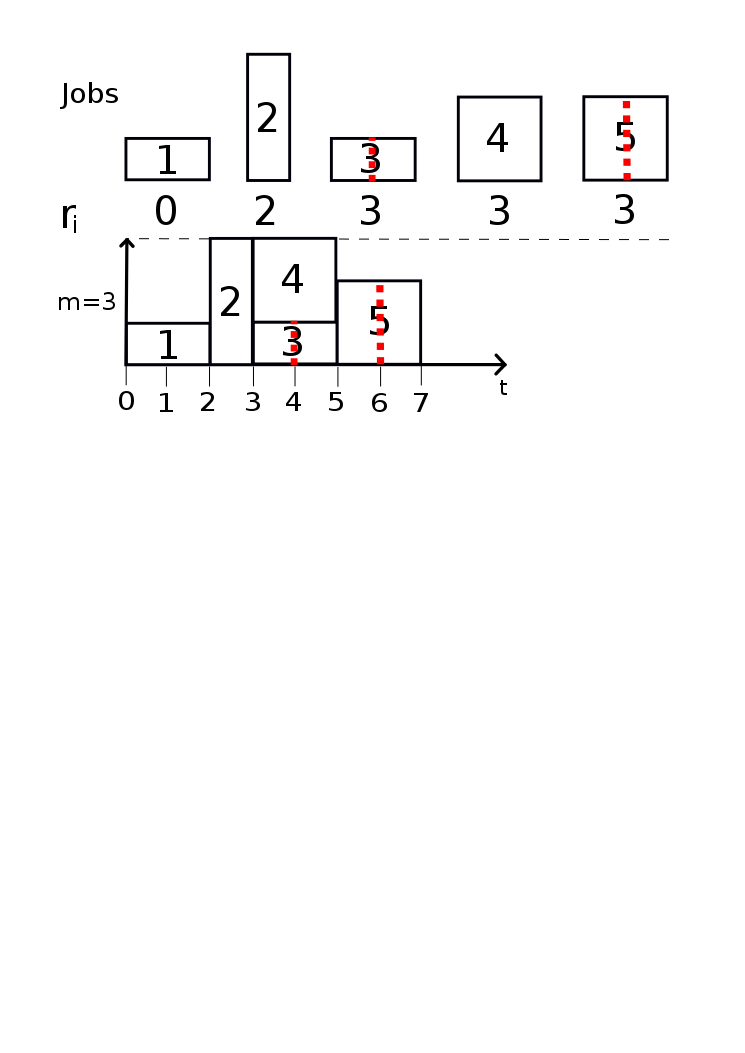
\includegraphics[width=\textwidth]{uncertain2.png}
          \caption{Caption}
          \label{fig:online2_png}
  \end{figure}

\end{frame}




\begin{frame}
  \frametitle{Optimization under Uncertainty}
  \centering
  \begin{tabular}{ll}
    \pause Robust Optimization & \pause Stochastic Programming &
    & \ \ \ + Input Modeling &
    \pause 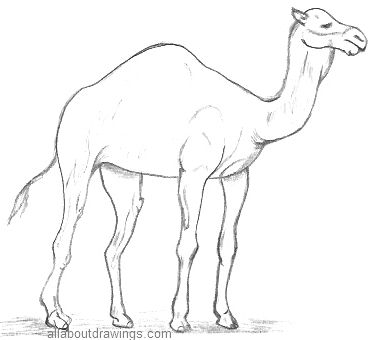
\includegraphics[width=.3\textwidth]{camel.jpg}& \pause 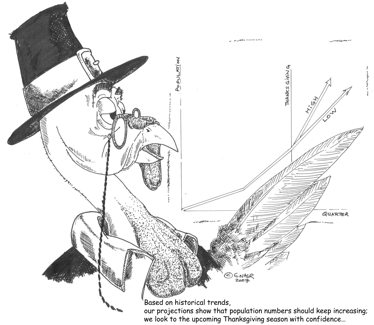
\includegraphics[width=.3\textwidth]{turkey.png} &
  \end{tabular}
\end{frame}

\begin{frame}
  \frametitle{The FCFS algorithm}
  \begin{figure}[H]
          \centering
          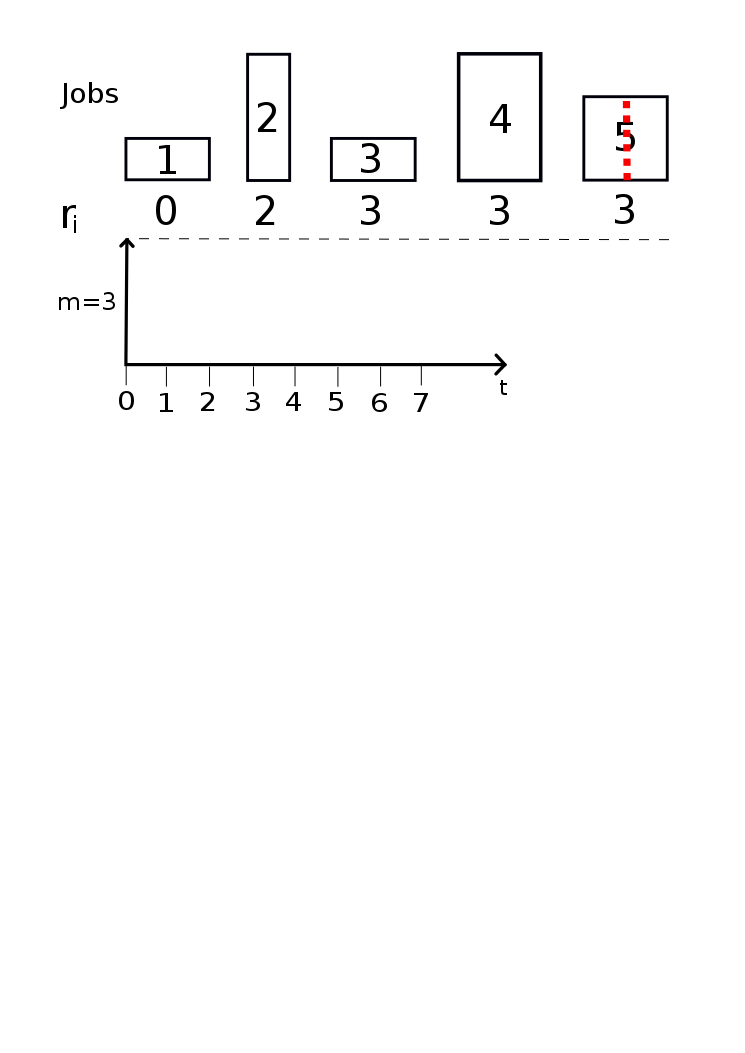
\includegraphics[width=\textwidth]{FCFS0.png}
          \caption{}
          \label{fig:fcfs0_png}
  \end{figure}

\end{frame}

\begin{frame}
  \frametitle{The FCFS algorithm}
  \begin{figure}[H]
          \centering
          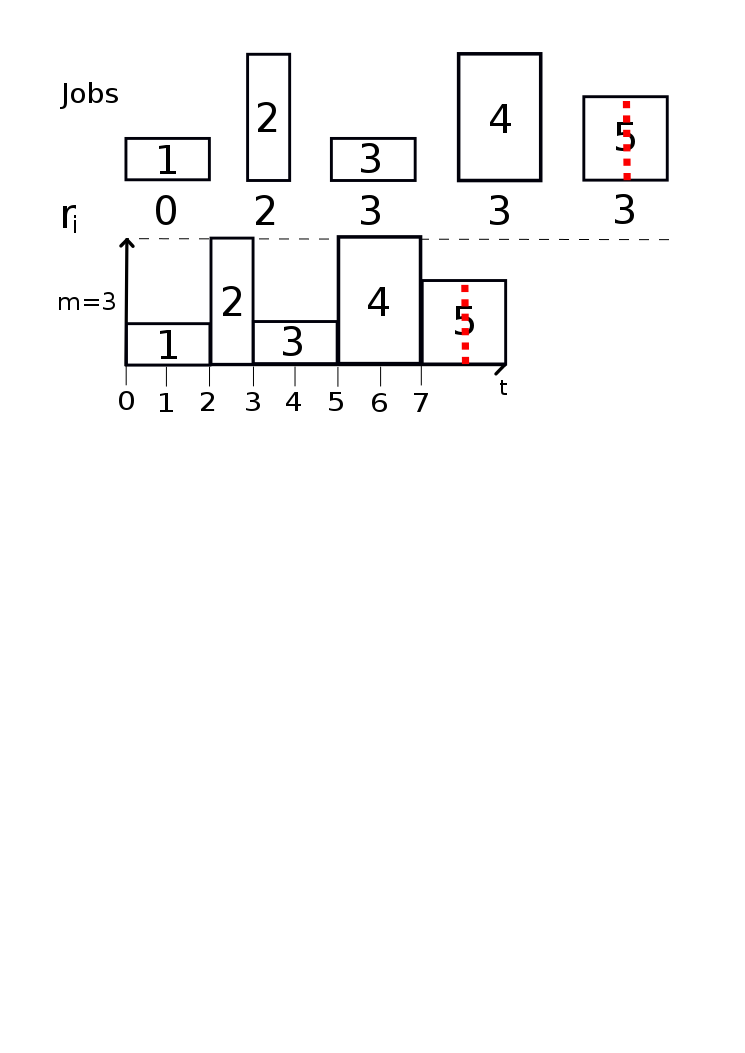
\includegraphics[width=\textwidth]{FCFS.png}
          \caption{}
          \label{fig:fcfs_png}
  \end{figure}

\end{frame}

\begin{frame}
  \frametitle{FCFS with EASY(conservative) backfilling}
  \begin{figure}[H]
          \centering
          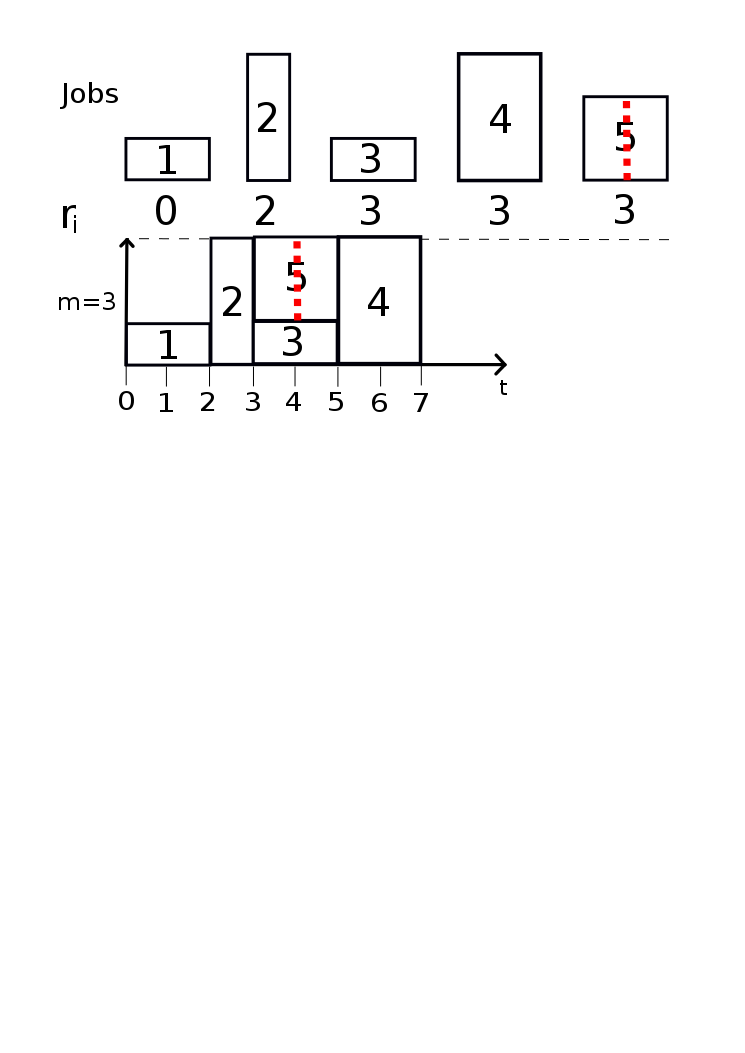
\includegraphics[width=\textwidth]{FCFSb.png}
          \caption{}
          \label{fig:fcfs_png}
  \end{figure}

\end{frame}

% section introduction (end)

\section{Runtime Prediction}
\label{sec:runtime_prediction}
\begin{frame}
  \frametitle{Runtime Prediction}
  Problem Statement:
  How to best Predict the Runtime of a job on a given system?
  \begin{figure}[H]
          \centering
          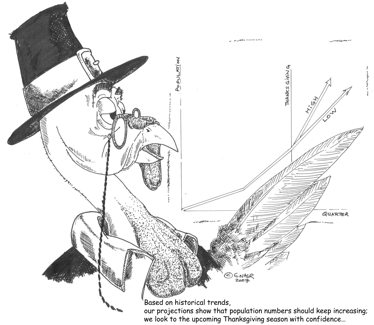
\includegraphics[width=0.2\textwidth]{turkey.png}
          \label{fig:turkey_png}
  \end{figure}
\end{frame}

\begin{frame}
  \frametitle{Nature of the Prediction}
%\usepackage{subcaption}
\begin{itemize}
  \item Single-valued?
  \item Probability distribution?
  \item Confidence Interval?
\end{itemize}
\end{frame}

\begin{frame}
  \frametitle{Nature of the Prediction}
%\usepackage{subcaption}
\begin{itemize}
  \item \textbf{Single-valued}
  \item Probability distribution
  \item Confidence Interval
\end{itemize}
\end{frame}

\begin{frame}
  \frametitle{Hypotheses on the Runtime}
  \begin{itemize}
    \item Independent and identically distributed?
    \item Is it dependent on job characteristics?
  \end{itemize}
\end{frame}

\begin{frame}
  \frametitle{Hypotheses on the Runtime}
  \begin{itemize}
    \item Independent and identically distributed? \textbf{No.}
    \item Is it dependent on job characteristics? \textbf{Yes.}
  \end{itemize}
\end{frame}


\begin{frame}
  \frametitle{State of the Art}

  \centering
  A very popular predictor:
  \[
    p_i^u =\frac{p_{i-1}^u+ p_{i-2}^u}{2}
  \]
  Baseline for evaluating our method.

\end{frame}


% section runtime_prediction (end)

\section{Random Forest Regression}
\label{sec:predicting_runtime_with_random_forests}
\begin{frame}
  \frametitle{Our Approach}
  Machine Learning: Regression problem. \\
  \pause
  Build vectors containing:
  \begin{itemize}
      \pause
    \item Job characteristics (e.g., required time and nodes)
      \pause
    \item Status of the system (e.g., day of the week)
      \pause
    \item Characteristics of the last jobs of this user (e.g., the baseline)
  \end{itemize}
  \pause
  Perform Regression using the Random Forest algorithm.
\end{frame}


\begin{frame}<1>[label=rf]
  \frametitle{Random Forests}
  \begin{itemize}
    \item Training: \begin{itemize}
        \item Randomly partition the training data.
        \item Learn a decision tree on each subset.
      \end{itemize}
    \item<2> Predict a value by averaging the results from all the decision trees.
  \end{itemize}
\end{frame}

\begin{frame}
  \frametitle{Decision Tree Learning}
  \pgfdeclarelayer{background}
  \pgfsetlayers{background,main}

  \tikzstyle{vertex}=[circle,fill=black!25,minimum size=20pt,inner sep=0pt]
  \tikzstyle{selected vertex} = [vertex, fill=red!24]
  \tikzstyle{edge} = [draw,thick,-]
  \tikzstyle{weight} = [font=\small]
  \tikzstyle{selected edge} = [draw,line width=5pt,-,red!50]
  \tikzstyle{ignored edge} = [draw,line width=5pt,-,black!20]
  \begin{figure}
    \[
      X=
      \left(
        \begin{array}{c}
          x \\
          y
        \end{array}
      \right)
      , (\alpha,\beta,a,b,c) \in \mathbb{R}^5
    \]
    \begin{tikzpicture}[->,
        scale=1.8,
        >=stealth',
        shorten >=1pt,
        %auto,
        node distance=3cm,
        thick,
        on grid,
        square/.style={draw,font=\sffamily\Large\bfseries}
      ]
      \node[vertex] (d) at (1,2) {};
      \node[vertex] (va) at (0,1) {};
      \node[vertex] (vb) at (2,1) {a};
      \node[vertex] (vc) at (-1,0) {b};
      \node[vertex] (vd) at (1,0) {c};
      \path[every node/.style={fill=white}]
      (d)
      edge node {$x>\alpha$} (vb)
      edge node {$x\leq\alpha$} (va)
      (va)
      edge node {$y>\beta$} (vc)
      edge node {$y\leq\beta$} (vd);
    \end{tikzpicture}
    \caption{A decision tree for predicting the value of $X$.}
  \end{figure}

\end{frame}


\againframe<2>{rf}
% section predicting_runtime_with_random_forests (end)

\section{Preliminary Results}
\label{sec:section_name}
\begin{frame}
\frametitle{Experiments}

\centering
On the CURIE log:

The features are extracted with the SimPy discrete event simulation package.

The RF is trained on the CURIE log using the first 80\% of the jobs, using the Scikit-Learn package.

\end{frame}
\begin{frame}
\frametitle{Results: Absolute Error Distribution}
\begin{figure}[H]
        \centering
        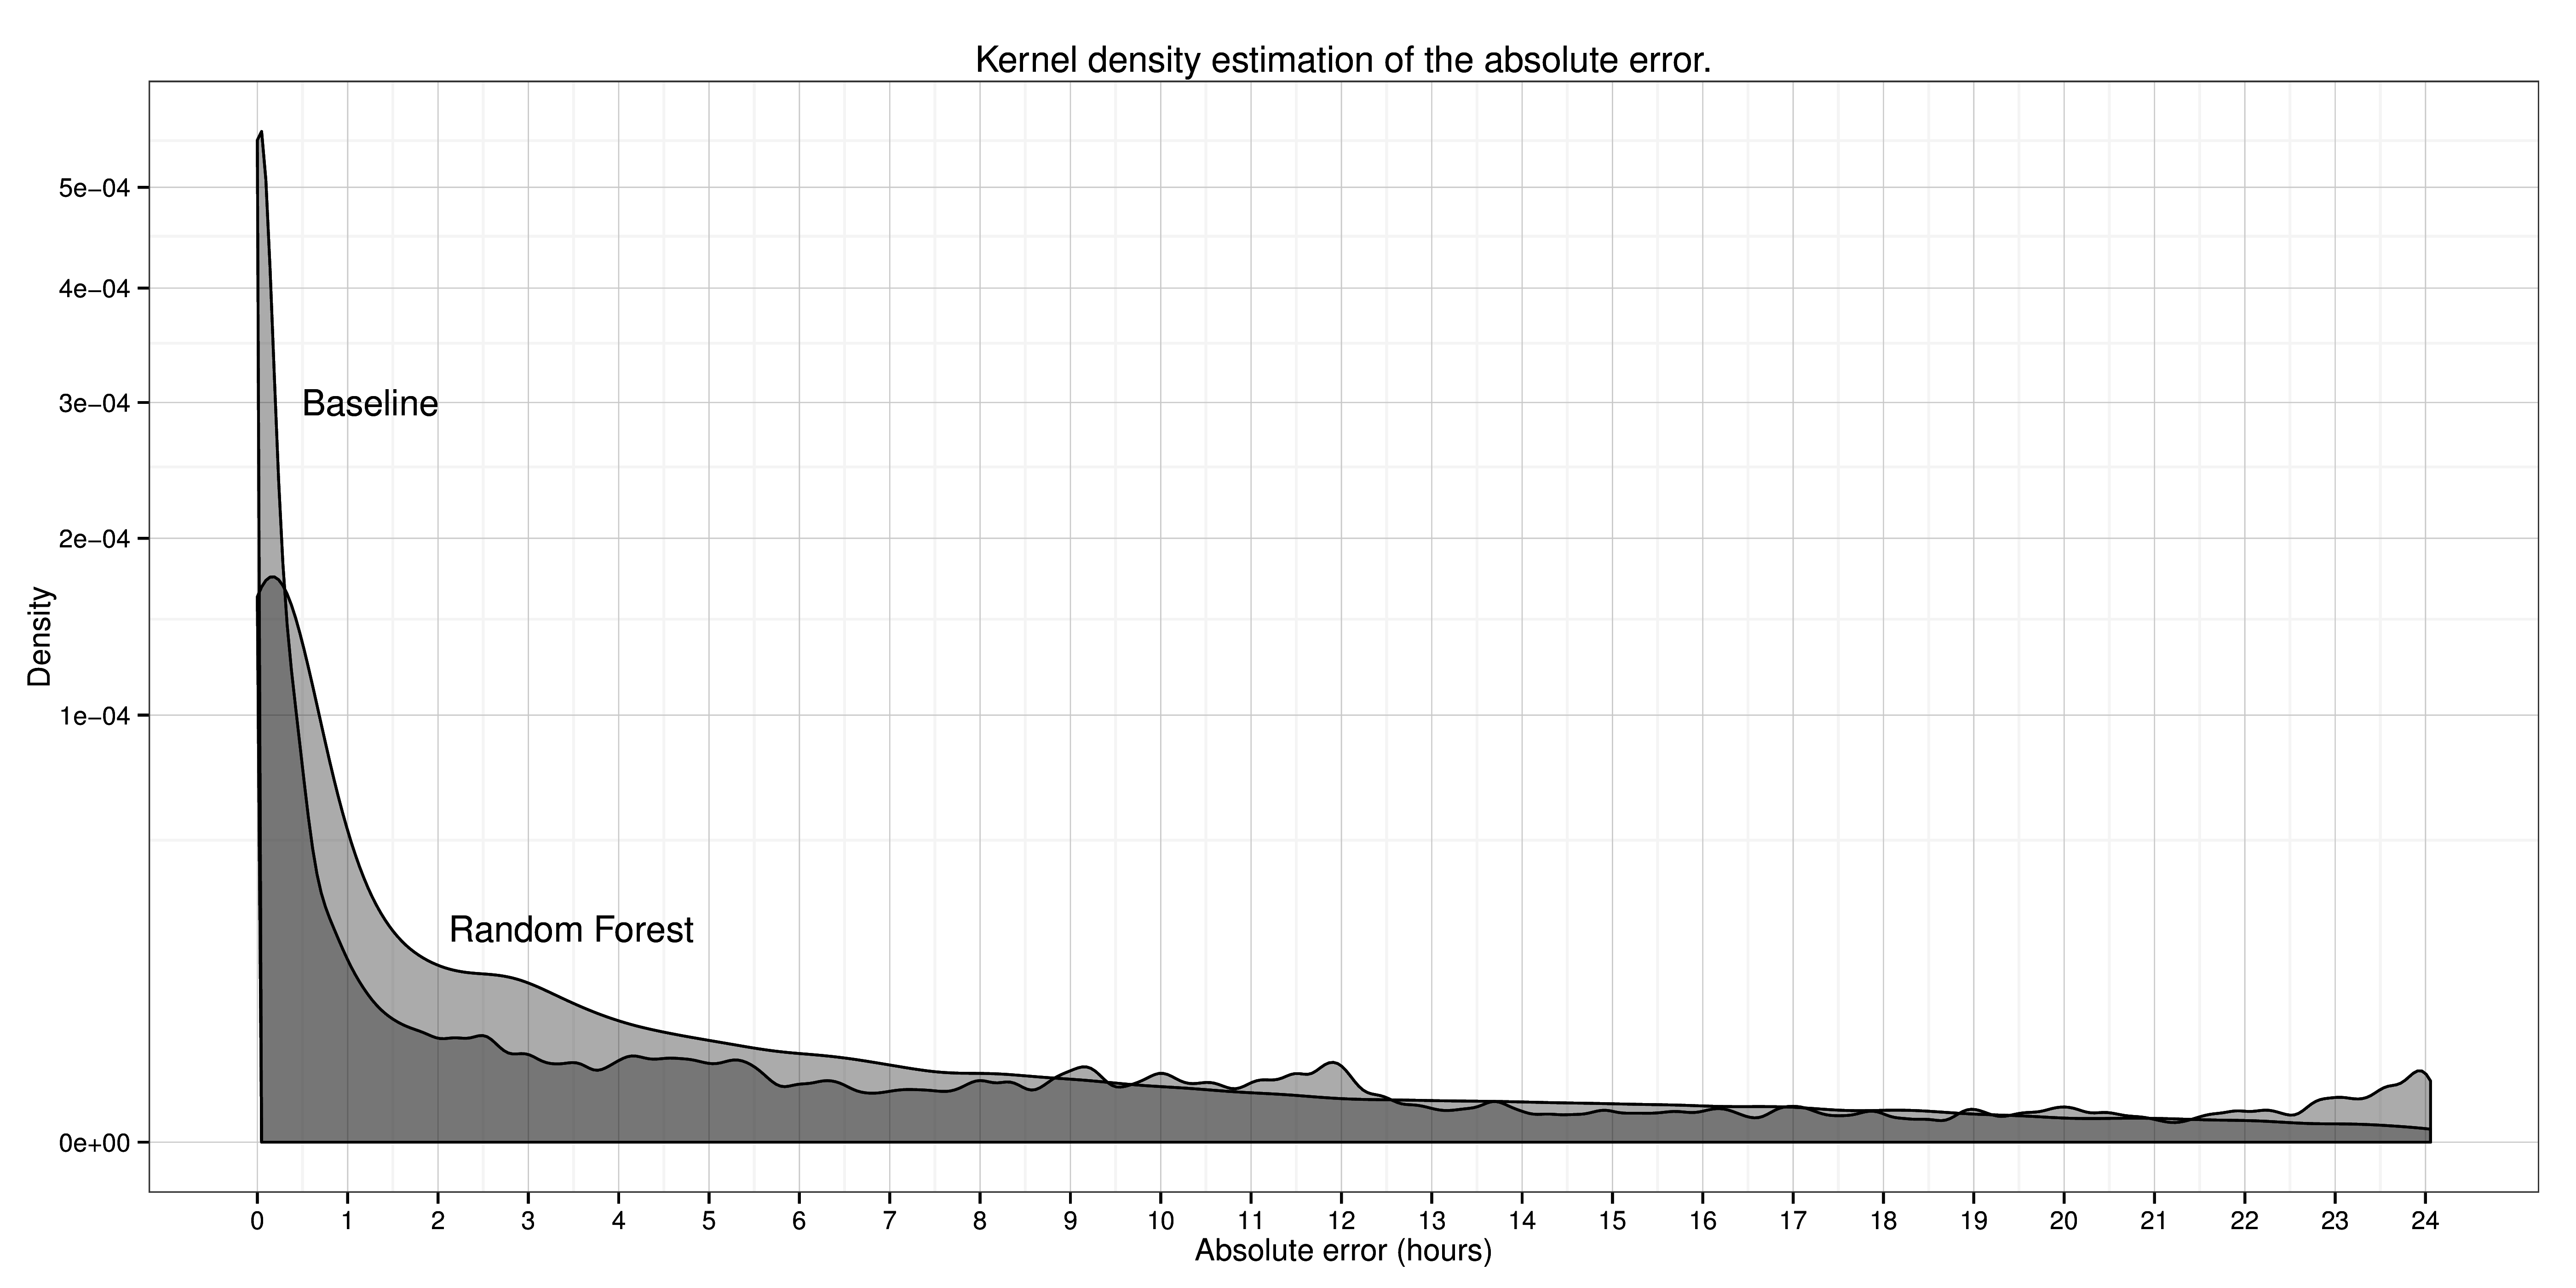
\includegraphics[width=\textwidth]{../report/error.png}
        \label{fig:_report_error_png}
\end{figure}
\end{frame}

\begin{frame}
\frametitle{Results: metrics}

  \begin{table}[ht]
    \centering
    \begin{tabular}{|l|l|l|}
      \hline
      %Measure & MSE measure ($\mbox{s}^2$)   \\
      Measure & Baseline & Random Forest &
      \hline
      MSE & \num{198497515} & \num{158202218} &
      \hline
      MAE & \num{4680.836} & \num{5551.237} &
      \hline
      Standard Error& \num{53.12812} & \num{45.12378} &
      %\hline
      %Random Forest & \num{158202218}\\
      \hline
    \end{tabular}
      \label{fig:lsq}
    \end{table}


\end{frame}
% section section_name (end)

\section{Perspectives}
\label{sec:perspectives}
\begin{frame}
\frametitle{Perspectives}

\begin{itemize}
\item Online Algorithm
\item More datasets, more features.
\item Sensitivity analysis, objective/cost functions.
\end{itemize}

\end{frame}

% section perspectives (end)

\section*{End}
\begin{frame}

  \Huge{\centerline{Thank you!}}
\end{frame}

\end{document}
